%\hypertarget{estilo:capitulo}{}
%%%%%%%%%%%%%%%%%%%%%%%%%%%%%%%%%%%%%%%%%%%%%%%%%
\section{Materials and method}\label{refmeto}
\subsection{Study Area}
This project admits as a study area the region of S�o Paulo inserted in the hydrographic basin of the River Tamanduate� (Figure \ref{fig:area_estudo}).
This basin has an area of $\SI{323}{\kilo \meter ^2}$ and extends to the hydrographic basins of the Pinheiro, Guai�, Aricanduva and C�rrego de Tapuap� rivers. This area was defined from the vicinity of a rain gauge, according to a spatial radius of \SI{2000}{\meter}, which encompasses different flooding regions, available Tweets and a meteorological radar cell.

\begin{figure}[H]
	\centering
	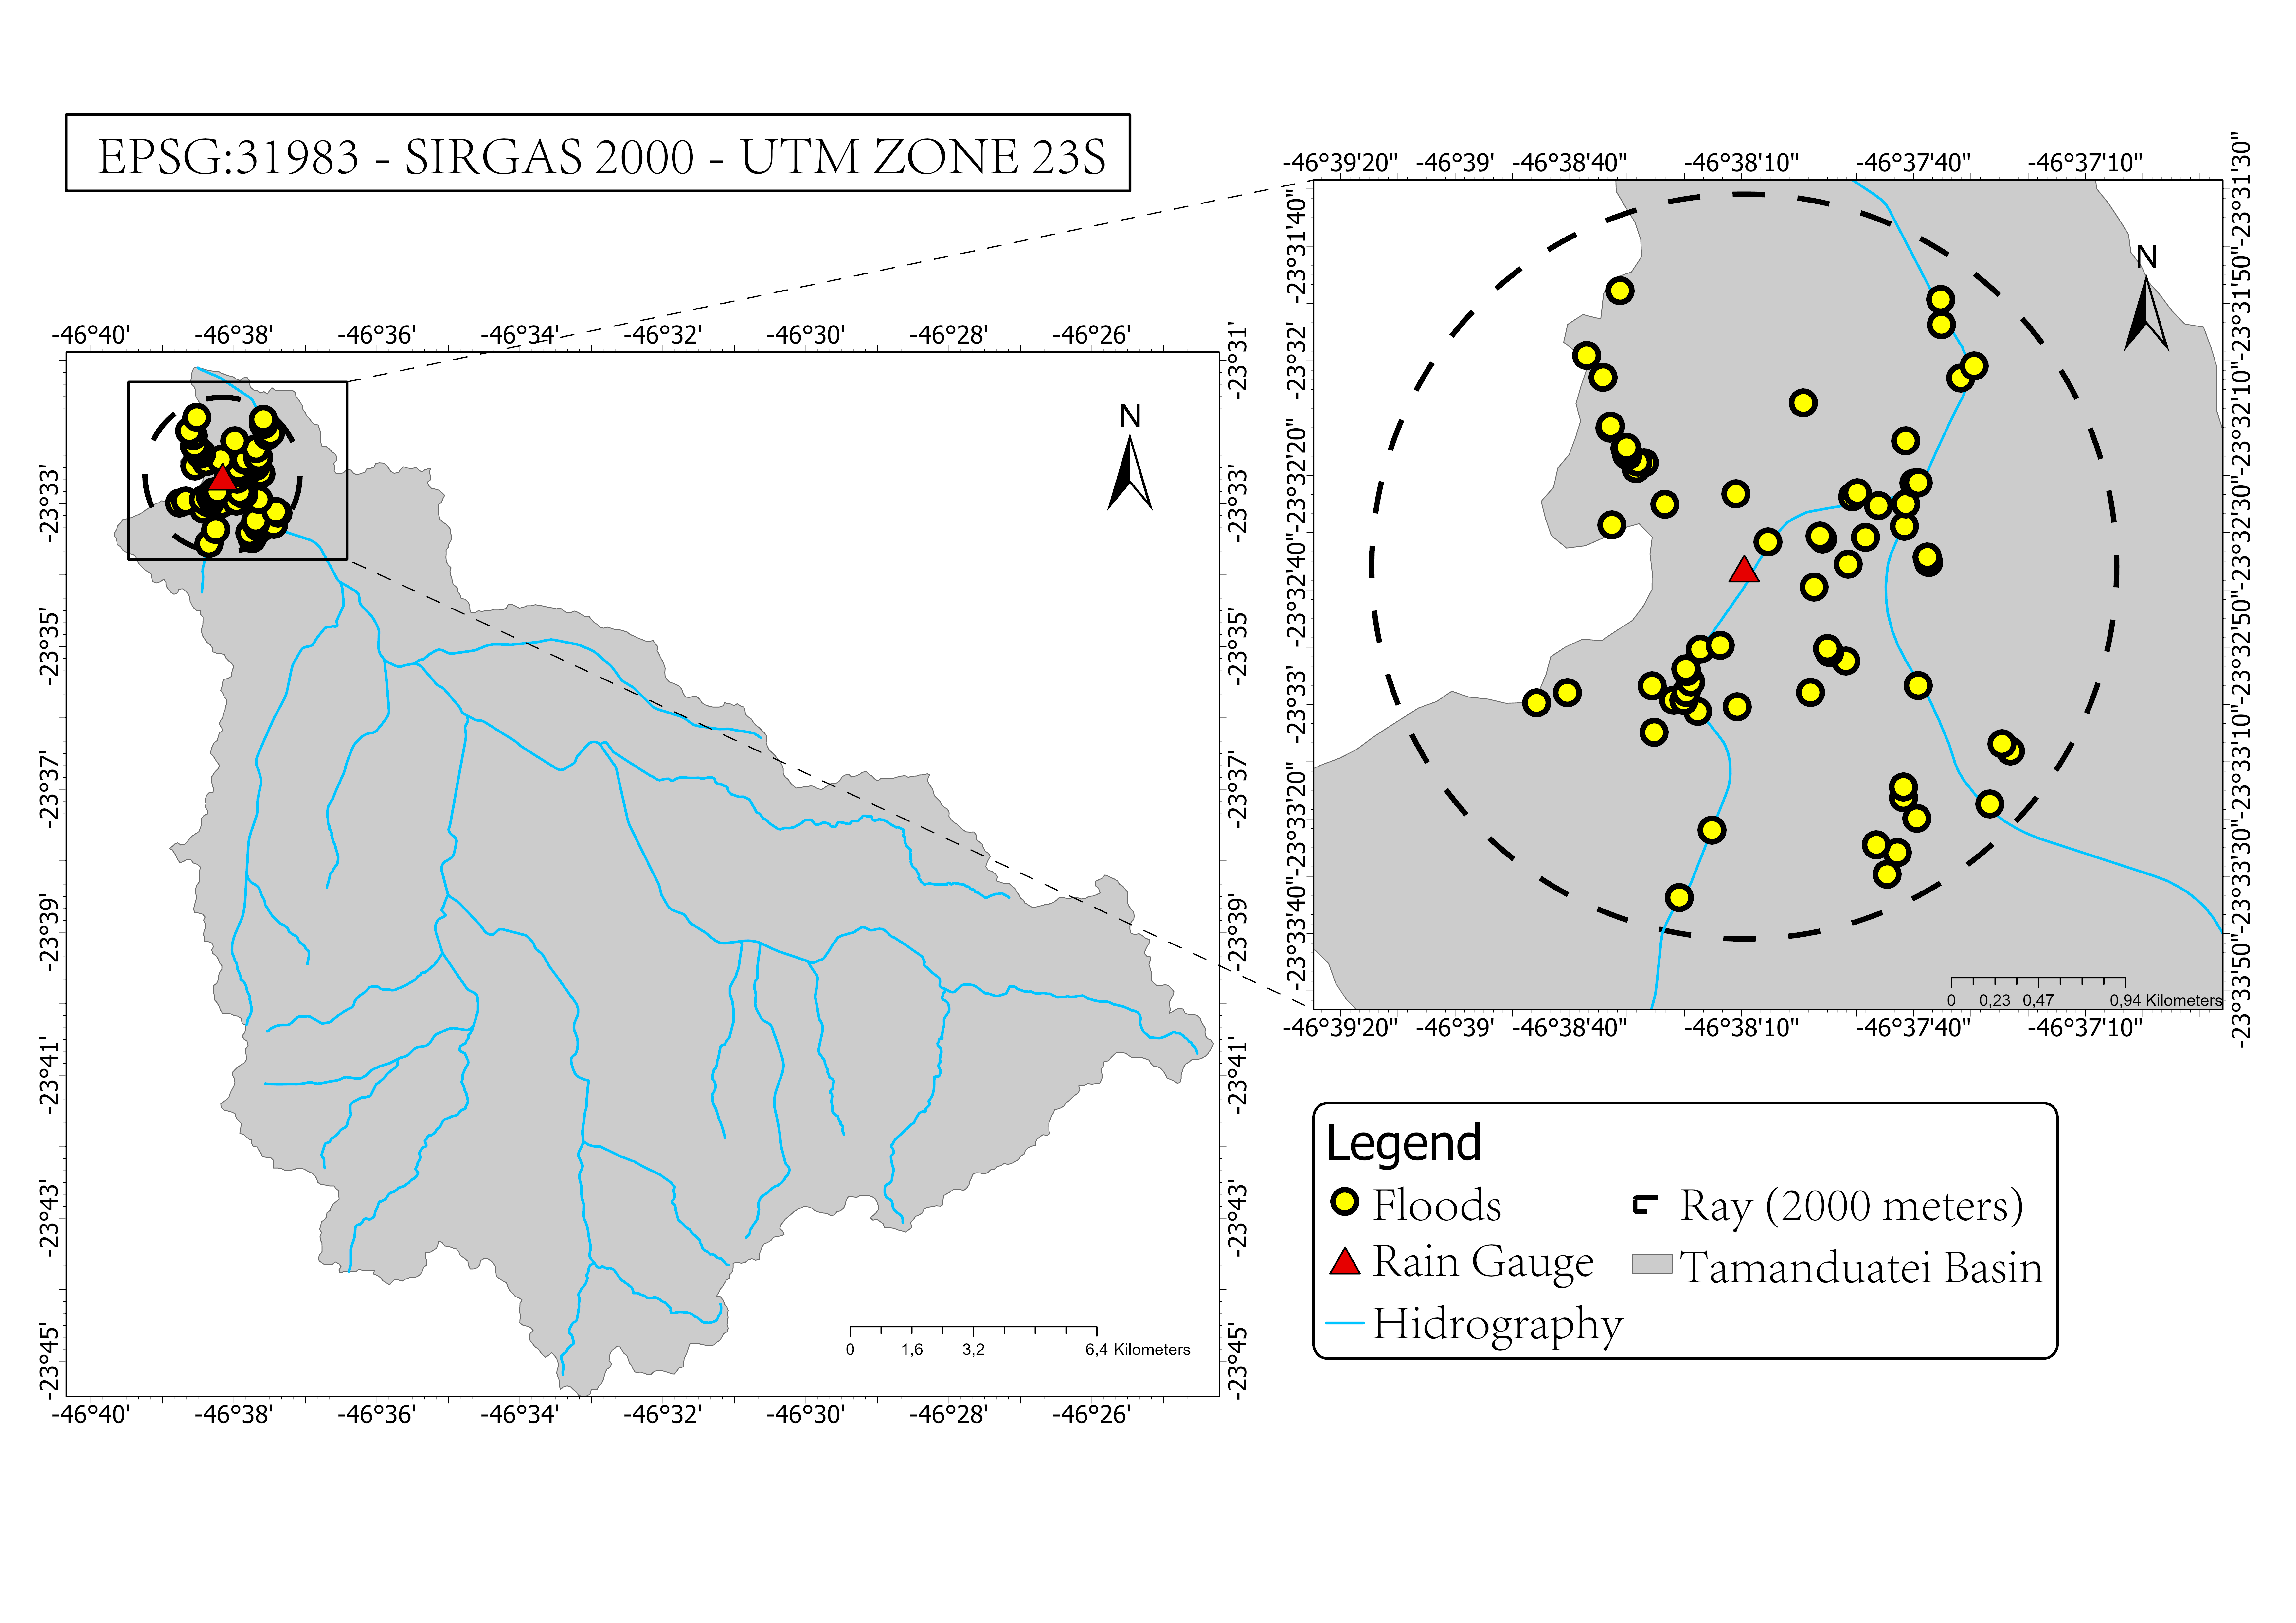
\includegraphics[scale=0.2]{figs/layout33.png}
	\caption{Study Area}
	\label{fig:area_estudo}
\end{figure}

\subsection{Data and tools}
Twitter data were extracted through an API (\textit{Application Programming Interface}) provided by the social network itself. The pluviometric data are collected from the pluviometer $\#833A$, belonging to the National Center for Alerts and Natural Disasters (CEMADEN), which are made publicly available by the institution.
The historical series of flooding in the study area is available through CEMADEN.

The data from the meteorological radar were extracted by a station located in the city of S�o Roque. This equipment, %belongs to CEMADEN and currently
maintained by the Department of Airspace Control (DECEA), it monitors displacement, action of clouds and instability nuclei, measuring the volume of precipitation in a given location. Furthermore, this radar has a range of \SI{250}{\kilo \meter}, covering the entire metropolitan region of S�o Paulo. The radar product used is called CAPPI (\textit{Constant Altitude Plan Position Indicator}),  which has a spatial resolution of approximately \SI{1}{\kilo\meter} and a temporal resolution of 10 minutes. For the conversion of reflectivity (dBZ) into separation rate (mm/h) the Marshall-Palmer ratio \cite{marshall1948mc} will be used, and then represented as ``daily accumulated''.

The development of the project will be guided by programming via the \textit{Python} language. The manipulation, filtering and processing of data will be supported by the \textit{Pandas} \cite{vanderplas2016python} and \textit{Numpy} \cite{mckinney2012python} libraries.

For the application of statistical tests, the \textit{Scipy} \cite{virtanen2020scipy} library will be used. Finally, necessary database operations will be performed with the support of the Geographic Information System \textit{QGIS} \cite{samela2018gis}
%Similarly, the classification methods used in the research (i.e., SVM, RF and MLP) will be obtained from the Scikit-Learn library \cite{pedregosa2011scikit}.



\subsection{Method in the first project}\label{method}
Firstly, all geolocated tweets from January to March 2019 within a radius of 2000 meters were extracted through API. The centroid of this ray is located in pluviometer 857A in S�o Paulo and the coordinates of this place can be found on the website of the institution CEMADEN. The data extracted through the Twitter API, uses the UTC format to inform the day and time of posts. Therefore, in the pre-processing of the tweets data, the date-time was converted from UTC for the Am�rica/S�o Paulo region. Also, to facilitate visualization and optimize the data, some unnecessary columns were removed. Finally, the date was delimited for the analyzed time window.


With the data from the social network, the filtering of tweets was carried out from a list of words separated as associated phenomena such as meteorological (METEO) and hydrological (HIDRO) \ref{table:tabelalista}.


\begin{table}[ht]
	\centering
	\caption{List of keywords.}\label{table:tabelalista}
	\begin{tabular}{ccccc}
		\hline 
		\multirow{2}{*}{METEO} & chuva & rain & temporal & lightning\tabularnewline
		& rainbow & raio & precipitacao & trov�o\tabularnewline
		\hline 
		\multirow{2}{*}{HIDRO} & alagado & alagamento & enchente & \tabularnewline
		& inundacao & enxente &  & \tabularnewline
		\hline 
	\end{tabular}
	% 		\begin{tabular}{c|c}
	% 			\hline
	% 			METEO & HIDRO \\ \hline
	% 			chuva & alagado \\
	% 			rain & alagamento \\
	% 			temporal & enchente \\
	% 			lightning & enxente \\
	% 			trov�o & inundacao \\
	% 			rainbow & - \\
	% 			raio & - \\
	% 			precita��o & - \\ \hline
	% 		\end{tabular}	
\end{table}
From the analysis of the time of occurrence of the floods using Microsoft Excel, a large portion of the floods occur between 4 pm and 8 pm. Therefore, the tweets were filtered from the list of words (Table \ref{table:tabelalista}), and in the time frame from 4:00 pm to 8:00 pm. The floods were processed through and filtered only to those belonging to the analyzed time interval.

The frequency of words in the METEO and HYDRO list was also generated, separating it into two data series, number of times of occurrence in days with flooding and days without flooding. This binary classification allowed the generation of Boxplots.


From the two series mentioned above, the MannWhitney non-parametric statistical test was applied to verify whether there is statistical relevance in the difference between the two series.

Complementary, Google Maps' photos of the study area show the topography of the places.
\subsection{Method in the second project} \label{secondmethod}
Based on the results of the Mann Whitney test, it was possible to use new data sources by integrating with the tweets. So similarly, tweets were collected via the API. To filter the posts for the context of flooding and rain, the words 'chuva', 'chove', 'chuvoso' and 'chuvosa' were used. These terms, according to \cite{de2021effect}, are less temporally and spatially volatile and are commonly used in the city of S�o Paulo to refer to the phenomena of rain and flooding. Any tweets that contain one of the above words are selected and counted for the day the post was sent by the user. Then, these posts are aggregated for each of the days of the analyzed time frame. 

Data from the 833A pluviometer were extracted from the website of the CEMADEN institution. The files containing the equipment information are found separated by month and measurements of all other rain gauges. In the primary treatment of the data, the files were concatenated and unified in a single DataFrame file, later only the measurements of the 833A rain gauge were filtered. This equipment, in times of absence of rain, records the information once in an hour, otherwise, in the detection of precipitation it starts measuring the rain every 10 minutes. Therefore, to analyze the rainfall data, the accumulated rainfall was calculated every 10 minutes for each day.

Radar data measurements are already processed and the information is found with the daily rainfall accumulation in a given cell. These cells comprise each of the rain gauge points. Therefore, values were extracted only from the point coinciding with the 833A pluviometer.

The flooding data was thoroughly reviewed by a member of the CEMADEN team. This information comes from meteorological and hydrological monitoring institutions. The outbreak of a flood is recorded from the moment there is an obstruction of a road due to accumulation of water and precipitation. Data are primarily found records of flooding throughout the entire Tamanduate� Basin and for the entire year of 2019. The day, time, duration, street name, latitude, longitude, start and end time of the flood are recorded in the file.

For the processing of the flooding data, geoprocessing tools in QGIS were used. First, a circumference of radius \SI{2000} {\meter} around the 833A rain gauge was created using the Buffer algorithm. Soon after, through the intersection algorithm between layers, only the floods belonging to the circle created by the Buffer were selected. The data were then delimited for the time window analyzed and the occurrences of flooding per day were counted.

With the processed data in hand, each of the attributes was integrated into a single DataFrame through the Merge function. In this table, all attributes are organized by the index that corresponds to the date, and each of the corresponding columns accumulated rainfall in the pluviometer and radar, frequency of tweets and number of occurrences of flooding.

To explore the data and verify the relationships between the attributes, the data were plotted as a function of the time window in a single graph. less frequent flooding. For more accurate inferences, Pearson and Spearman correlations were calculated. In selecting the appropriate correlation algorithm, the Shapiro Wilk test was used to determine whether the attributes followed a normal distribution, that is, parametric or non-parametric.

After determining the type of statistical distribution, the appropriate correlation algorithm was defined. Thus, inferences were made relating the attributes with the occurrence of flooding.



%The initial design of this research proposal consists in the use of time series of floods, Tweets, data recorded by rain gauge and meteorological radar, in order to build a method for forecasting flood events.
%An overview of the proposal is illustrated in Figure~\ref{fig:metodologia}.

%\begin{figure}[H]
%	\centering
	%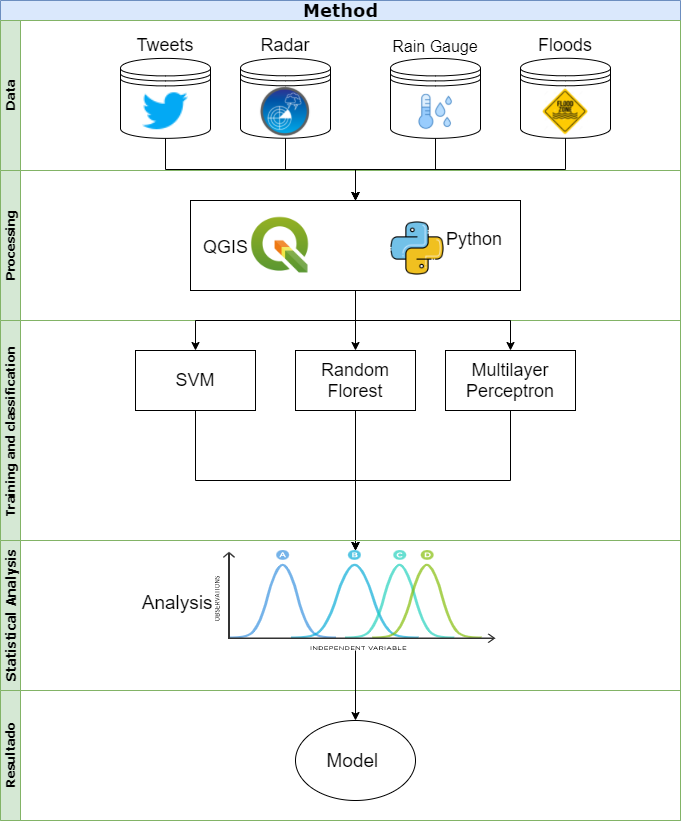
\includegraphics[width=0.6\textwidth]{figs/metodolog.png}
	%\caption{Method}
	%\label{fig:metodologia}
%\end{figure}

%Initially, information on the number of filtered Tweets, precipitation values according to radar and rain gauge, and whether there was flooding in the analyzed days will be organized in a single file. In a second moment, this data will be submitted to the SVM, RF and MLP methods. In this phase, different subsets of attributes will be verified among the available ones. An initial division of this base will be admitted, in the proportion $\displaystyle \frac{2}{3} \sim \frac{1}{3}$ for the purposes of training and testing the models. 
%The classifications to be carried out will comprise the classes ``flooding'' or ``non-flooding'', whose accuracy will be measured by the basis of tests using measures such as kappa coefficient, F1-Score and cross validation procedure.

%Subsequently, statistical tests on the significance of the results will indicate the most relevant method and attributes for building a flood warning system. 